\documentclass[tikz,border=3pt]{standalone}
\usepackage[utf8]{inputenc}
\usepackage[T1]{fontenc}
\usepackage{lmodern}
\renewcommand{\familydefault}{\sfdefault}
\usepackage{sansmath}\sansmath
\usepackage{chemfig}
\usepackage{pgfplots}\pgfplotsset{compat=1.18,/pgf/number format/use comma,/pgf/number format/1000 sep={.}}
\usetikzlibrary{arrows.meta,calc,positioning,decorations.pathmorphing,patterns}
% paleta del sitio
\definecolor{nar}{HTML}{E8680C}\definecolor{narc}{HTML}{FFB35C}\definecolor{hielo}{HTML}{FFF3E8}
\definecolor{tinta}{HTML}{1D1D1F}\definecolor{gris}{HTML}{6E6E73}\definecolor{lila}{HTML}{7C5CF0}
\definecolor{azul}{HTML}{2F6FD6}\definecolor{menta}{HTML}{17A673}\definecolor{coral}{HTML}{E8342A}
\begin{document}
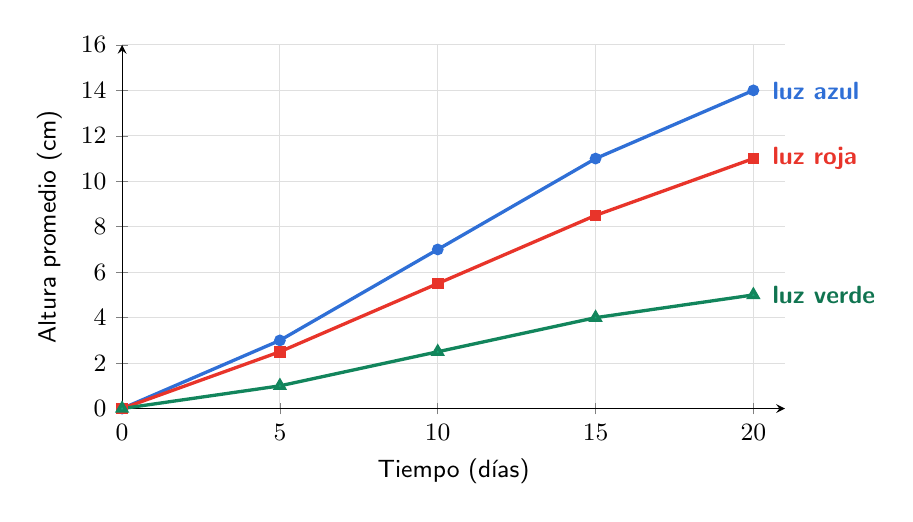
\begin{tikzpicture}[font=\small]
\begin{axis}[width=10cm,height=6.2cm,axis lines=left,xmin=0,xmax=21,ymin=0,ymax=16,xtick={0,5,...,20},ytick={0,2,...,16},
  grid=major,grid style={gray!25},xlabel={Tiempo (días)},ylabel={Altura promedio (cm)},clip=false]
\addplot[azul,very thick,mark=*,mark options={fill=azul,scale=0.75}] coordinates {(0,0)(5,3)(10,7)(15,11)(20,14)};
\addplot[coral,very thick,mark=square*,mark options={fill=coral,scale=0.75}] coordinates {(0,0)(5,2.5)(10,5.5)(15,8.5)(20,11)};
\addplot[menta!80!black,very thick,mark=triangle*,mark options={fill=menta,scale=0.9}] coordinates {(0,0)(5,1)(10,2.5)(15,4)(20,5)};
\node[azul,font=\small\bfseries,anchor=west] at (axis cs:20.3,14) {luz azul};
\node[coral,font=\small\bfseries,anchor=west] at (axis cs:20.3,11) {luz roja};
\node[menta!70!black,font=\small\bfseries,anchor=west] at (axis cs:20.3,5) {luz verde};
\end{axis}
\end{tikzpicture}
\end{document}
